% SCOPE preprint -- revtex4-2, single-column preprint format
% Compile with pdfLaTeX. Requires figure1.pdf in the same directory.
\documentclass[aps,pre,preprint,superscriptaddress,nofootinbib,floatfix]{revtex4-2}

\usepackage{amsmath,amssymb}
\usepackage{graphicx}
\usepackage{booktabs}
\usepackage[T1]{fontenc}
\usepackage{siunitx}

\newcommand{\tb}{\tau_{\mathrm{border}}}
\newcommand{\ti}{\tau_{\mathrm{diss}}}

\begin{document}

\title{Seed geometry predicts the onset of near-boundary gradient dissipation in a spherical Gray--Scott system}

\author{{\L}ukasz Ciesielski}
\affiliation{Independent Researcher}
\email{lukas.ciesielski@icloud.com}

\date{\today}

\begin{abstract}
We investigate how the spatial geometry of initial seeding controls the first-passage statistics of a near-boundary gradient-dissipation proxy in a three-dimensional Gray--Scott reaction--diffusion system on a spherical domain with no-flux boundary conditions. Under these boundary conditions there is no net flux through the wall; the observable is the local gradient-squared dissipation $D = D_u|\nabla u|^2 + D_v|\nabla v|^2$ in a boundary-adjacent shell, and $\tb$ is the first passage of this pattern-associated gradient cost to that shell---not a transport of material across the boundary. Three seed topologies of equal volume---central concentration, sub-boundary shell, and space-filling distribution---are systematically compared using pre-registered acceptance criteria and Kaplan--Meier survival analysis of $\tb$.
Across two grid resolutions ($192^3$ and $288^3$, combined $n=28$ per topology) we find that the ordering distributed $<$ shell $<$ central is preserved with median $\tb$ ratios spanning nearly one decade (up to $9.3\times$), stable across threshold choices of \SIrange{1}{50}{\percent} and yielding log-rank $p_{\mathrm{Holm}} \le 1.3\times10^{-6}$ for all pairwise contrasts on both scales. The per-run distributions are strongly degenerate for compact topologies, so the effect sizes---median ratios---rather than the $p$-values are the substantive result. Reproducibility was verified by independently seeded batches ($n=6+6$) run two weeks apart. The shell scale ratio $\tau(288^3)/\tau(192^3)=1.40$ falls within pre-registered bounds $[1.25,1.75]$, consistent with self-similar scaling for that topology. Against a parametric sensitivity yardstick $(F,k)\pm\SI{0.5}{\percent}$, the two contrasts involving the central topology exceed parametric noise by factors $3.1\times$ and $4.7\times$, while the shell--distributed contrast ($1.57\times$) is weak relative to parameter uncertainty.
A heuristic decomposition of the onset time into activation and transport phases indicates that the ordering reflects at least two distinct geometric mechanisms---plausibly including seed surface-to-volume---rather than radial distance alone.
The simulations show a robust association between seed geometry and the onset of a boundary-adjacent gradient-dissipation proxy under the specified Gray--Scott protocol, situating the result within Prigogine's dissipative-structure framework as a controlled numerical observation rather than a claim of boundary transport or rigorous entropy production.
\end{abstract}

\maketitle

\section{Introduction}

Dissipative structures---systems maintained far from thermodynamic equilibrium that develop and sustain local order at the expense of entropy export to their environment---constitute one of the central paradigms of nonequilibrium physics. Since the foundational work of Prigogine and Nicolis~\cite{prigogine1977,nicolis1971}, the entropy balance $dS = d_eS + d_iS$~\cite{degroot1984}, with internal production $d_iS>0$ offset by boundary exchange $d_eS<0$, has framed our understanding of how spatial organization emerges and persists in open systems, from chemical oscillators to living matter. Reaction--diffusion systems (RDS) remain the canonical testing ground for this framework~\cite{cross1993}, combining analytical tractability with rich spatiotemporal phenomenology.

The thermodynamic description of RDS has recently reached considerable rigor. Falasco, Rao, and Esposito~\cite{falasco2018} constructed nonequilibrium potentials for reaction--diffusion dynamics and decomposed the total entropy production rate into diffusive and reactive contributions, classifying Turing pattern formation as a genuine thermodynamic phase transition in the one-dimensional Brusselator. Complementarily, Liang \textit{et al.}~\cite{liang2024} recently introduced a thermodynamically consistent variational extension of the Gray--Scott model, recovering the classical two-species system as a limiting subsystem of a closed reaction network. Notably, Serna \textit{et al.}~\cite{serna2017} demonstrated that distinct pattern morphologies can carry identical relative entropy, suggesting that morphology and stationary thermodynamics may be decoupled. These studies share two limitations relevant here: they are formulated on one-dimensional domains, and they characterize stationary or persistent states rather than the transient kinetics by which structure reaches the system boundary. Whether the spatial arrangement of initial structure carries predictive power for the temporal statistics of near-boundary dissipation remains, to our knowledge, unexamined.

A complementary methodological tradition measures first-passage observables in dissipative and diffusive systems, from avalanche lifetime distributions in self-organized criticality~\cite{bak1987} to the contemporary analysis of Brownian first-passage times in spherical and shell-like geometries~\cite{grebenkov2020,grebenkov2022}. This literature provides mature statistical machinery---survival analysis, censoring, mean first-passage asymptotics---but has been applied almost exclusively to point-particle diffusion; the first passage of organized structure in a nonlinear RDS has not, to our knowledge, been treated with these tools. Reaction--diffusion dynamics on and within spherical domains is itself an active subject: weakly nonlinear analysis predicts which Turing modes emerge in a ball~\cite{villarsepulveda2024}, and the role of initial conditions in three-dimensional pattern selection has begun to be mapped~\cite{bentahar2023}. These studies characterize which stationary patterns form, not the temporal statistics by which structure reaches the boundary.

Here we combine both threads. We study the three-dimensional Gray--Scott system~\cite{pearson1993,gray1984} on a spherical domain with no-flux boundary conditions and ask whether the geometry of initial seeding---central concentration, sub-boundary shell, or space-filling distribution, at equal seeded volume---predicts the first passage of a near-boundary gradient-dissipation proxy, $\tb$. Because the boundary is reflecting, this is not transport of material across the wall but the arrival time of pattern-associated gradient cost at a boundary-adjacent shell. Using pre-registered acceptance criteria, Kaplan--Meier survival analysis with right censoring, and a parametric sensitivity yardstick separating geometric effects from working-point sensitivity, we find that seed geometry robustly orders these onset times across two grid resolutions. The protocol, including frozen evaluation criteria and pre-registered scaling bounds, was fixed before the confirmation runs; all raw data, analysis scripts, and the decision audit trail are publicly available.

The paper is organized as follows. Section~\ref{sec:methods} defines the model, the seeding topologies, and the observable $\tb$. Section~\ref{sec:protocol} describes the pre-registered confirmation protocol. Section~\ref{sec:results} presents the results across both grid scales, including the sensitivity yardstick. Section~\ref{sec:discussion} discusses interpretation, limitations, and directions for extending the analysis.

\section{Model and Methods}
\label{sec:methods}

\subsection{Model and domain}

We study the Gray--Scott reaction--diffusion system for two scalar fields $u(\mathbf{r},t)$, $v(\mathbf{r},t)$:
\begin{align}
\partial_t u &= D_u \nabla^2 u - uv^2 + F(1-u),\\
\partial_t v &= D_v \nabla^2 v + uv^2 - (F+k)v,
\end{align}
with $D_u=0.16$, $D_v=0.08$, $F=0.042$, $k=0.062$, integrated by explicit Euler stepping ($dt=0.18$) on cubic grids of $192^3$ and $288^3$ sites. The working point $(F,k)$ was selected in a pilot phase as the regime in which all three seeding topologies produce persistent, non-saturating patterns; it was frozen before confirmation runs. The computational domain is a sphere inscribed in the cubic grid, with no-flux (Neumann) boundary conditions enforced through a masked-Laplacian formulation. The Laplacian is evaluated as a 3D convolution with a boundary-corrected kernel; numerical equivalence of this implementation against a reference finite-difference version was verified to $\max|\Delta|=1.79\times10^{-7}$ (tolerance $10^{-6}$) on the target hardware. Details of the discretization and the equivalence gate are given in Appendix~\ref{app:laplacian}.

\subsection{Seeding topologies}

Three initial seeding topologies of equal seeded volume are compared: \textit{central} (a single ball at the domain center), \textit{shell} (a spherical layer beneath the boundary), and \textit{distributed} (randomized non-overlapping balls filling the domain). Seeded-volume matching across topologies is verified per run (match ratio $1.00\pm0.01$). At $192^3$ the shell thickness is $3.0$ voxels, yielding a seeded fraction of ${\approx}\SI{5.7}{\percent}$ for all topologies. At $288^3$ two variants are used: a self-similar shell (thickness $4.5$, preserving the \SI{5.7}{\percent} fraction; arm~$\mathrm{B}'$) and a fixed-thickness variant (thickness $3.0$, fraction ${\approx}\SI{3.8}{\percent}$; arm~C). The resulting confound between domain scale and seeded fraction in arm~C is deliberate and is addressed in the interpretation of scale ratios (Sec.~\ref{sec:fullc}). Two admissibility gates ensure no seed overlaps the boundary measurement shell or the inner core, preventing pre-loading of the observable (Appendix~\ref{app:gates}).

\subsection{Observable}

The primary observable is $\tb$: the first time the boundary dissipation rate reaches \SI{10}{\percent} of its own final value at the horizon $T$. The boundary dissipation rate is the region-averaged gradient-squared dissipation $D = D_u|\nabla u|^2 + D_v|\nabla v|^2$ over the shell $r\in[0.85R,R]$. This is a phenomenological analogue of the diffusive contribution to entropy production; it is \textit{not} the rigorous entropy-production rate of a thermodynamically consistent theory---Gray--Scott is not such a theory---but it tracks the same physical quantity, the spatial-gradient cost of maintaining structure, and is directly comparable across topologies. Its relation to the formal diffusive entropy-production rate of Falasco \textit{et al.}~\cite{falasco2018} is discussed in Sec.~\ref{sec:physinterp}. The per-run adaptive threshold normalizes across topologies with different asymptotic dissipation levels; we note this normalization acts \textit{against} the hypothesis that compact seeds are slower (topologies with low asymptotic near-boundary dissipation reach their own \SI{10}{\percent} more easily), making it conservative. Runs never reaching threshold are right-censored at $T$. Threshold stability is assessed secondarily over the range \SIrange{1}{50}{\percent}.

\subsection{Pre-registered protocol}
\label{sec:protocol}

Evaluation criteria were frozen before confirmation (CRITERIA~v2): per-arm validity gates (all runs alive, volume matching, fraction consistency, non-degenerate dissipation), pairwise log-rank (Mantel--Cox~\cite{mantel1966}) tests on Kaplan--Meier~\cite{kaplan1958} curves with Holm correction~\cite{holm1979}, and three disjoint verdicts (CONFIRMED / NEGATIVE / INCONCLUSIVE). Scaling bounds for the $288^3/192^3$ median ratio---$[1.25,1.75]$ for front-propagation transport, ${\le}1.15$ for homogenization---were pre-registered before arm~$\mathrm{B}'$ was run. Confirmation comprised arm~A ($192^3$, $n=16$ per topology), arm~$\mathrm{B}'$ ($288^3$, shell only, $n=12$), and arm~C ($288^3$, all topologies, $n=12$, executed as two independent batches two weeks apart). A parametric sensitivity yardstick---nine runs on a $3\times3$ grid of $(F,k)\pm\SI{0.5}{\percent}$ at fixed topology and seed---quantifies working-point sensitivity of $\tb$ for comparison against inter-topology effects. All runs used seeds 2000--2011 on dual NVIDIA T4 GPUs; the complete audit trail (frozen criteria, changelog, raw outputs) is available in the public repository.

\section{Results}
\label{sec:results}

\subsection{Primary arm: geometry orders onset times at $192^3$}

All 48 runs of arm~A ($n=16$ per topology) passed the validity gates: every run alive at horizon, seeded fractions \SIrange{5.71}{5.74}{\percent}, fill factors \numrange{0.619}{0.620} across topologies. Median first-passage times at the \SI{10}{\percent} threshold were $\tb = 360$ (distributed), $1350$ (shell), and $3330$ (central), giving median ratios of $9.3\times$ (central/distributed), $3.75\times$ (shell/distributed), and $2.47\times$ (central/shell)---a span approaching one decade. All pairwise log-rank contrasts are significant after Holm correction ($p_{\mathrm{Holm}}\le1.9\times10^{-7}$; Table~\ref{tab:logrank}), with no censored runs.

The per-run distributions are, however, strongly degenerate: at the \SI{10}{\percent} threshold all 16 central runs and all 16 shell runs yield an \textit{identical} $\tb$ (3330 and 1350 respectively), and 15 of 16 distributed runs give 360. Seed noise (amplitude 0.02) thus has negligible effect on the onset time for these topologies. This is direct evidence that the geometric effect is near-deterministic with respect to seed realization, but it also means the effective number of independent observations is smaller than the nominal $n$, so the log-rank $p$-values---while unambiguous about the ordering---overstate the statistical information available. We therefore treat the median ratios, not the $p$-values, as the substantive effect measure throughout. The ordering distributed $<$ shell $<$ central is preserved at every threshold in the \SIrange{1}{50}{\percent} range (Table~\ref{tab:threshold}), indicating the effect is not an artifact of the threshold choice.

\subsection{Scale control: pre-registered scaling bounds}

Arm~$\mathrm{B}'$ ($288^3$, shell, self-similar seeding at \SI{5.73}{\percent} fraction, $n=12$) yielded median $\tb=1890$, giving a scale ratio $\tau(288^3)/\tau(192^3)=1890/1350=1.40$---within the pre-registered self-similar-scaling bounds $[1.25,1.75]$ and far from the homogenization bound (${\le}1.15$). The ratio remains within bounds for thresholds \SIrange{5}{25}{\percent} ($1.62$, $1.40$, $1.28$), exceeding the upper bound only at \SI{1}{\percent} ($2.11$) and approaching the homogenization boundary at \SI{50}{\percent} ($1.19$), consistent with an early transient dominated by local activation and a late regime approaching quasi-stationarity, with self-similar front growth in the mid-transient where the primary threshold lies. This scaling test is established for the shell topology only, since $\mathrm{B}'$ preserves the seeded fraction only for shell.

\subsection{Full control arm: ordering replicates at $288^3$}
\label{sec:fullc}

Arm~C ($288^3$, all topologies, $n=12$, fixed shell thickness, seeded fraction \SIrange{3.81}{3.83}{\percent}) reproduced the complete ordering: $\tb = 855$ (distributed), $1890$ (shell), $4770$ (central), with all pairwise contrasts significant ($p_{\mathrm{Holm}}\le1.3\times10^{-6}$; Table~\ref{tab:logrank}) and threshold-stable across \SIrange{1}{50}{\percent}. The two halves of arm~C, executed as independent batches two weeks apart with disjoint seeds, produced statistically indistinguishable results (shell median $\ti=2745$ in both; medians of all topologies within \SI{1}{\percent}).

Scale ratios relative to arm~A are $1.40$ (shell) and $1.43$ (central)---both within the pre-registered bounds---and $2.25$ (distributed), exceeding the upper bound. The distributed excess is consistent with the deliberate fraction confound of arm~C (Sec.~\ref{sec:methods}\,B): at \SI{3.8}{\percent} seeded fraction, the distributed topology, whose onset relies on seeds already near the boundary, is the most sensitive to seed dilution. The self-similar arm~$\mathrm{B}'$ shows that when the fraction is preserved, the shell ratio scales cleanly; a self-similar variant for all topologies is a natural extension, and until it is run the central and distributed ratios cannot be read as clean scaling tests.

\subsection{Sensitivity yardstick: topological effect vs working-point noise}

The $(F,k)\pm\SI{0.5}{\percent}$ probe (nine points, fixed shell topology and seed, $192^3$) produced $\tb$ spread of 630 steps (range \numrange{1080}{1710}, median 1350), with fill factors \numrange{0.595}{0.643} confirming the probe remains within the working regime. Notably, $\tb$ varied almost exclusively along $k$, with negligible dependence on $F$. A wider $\pm\SI{2}{\percent}$ probe left the regime entirely (fill \numrange{0.51}{0.72}, spread 3060) and is reported only as a negative reference in the repository.

Against this yardstick, the inter-topology differences at $192^3$ are 2970 (central${-}$distributed, $4.7\times$), 1980 (central${-}$shell, $3.1\times$), and 990 (shell${-}$distributed, $1.57\times$); see Table~\ref{tab:yardstick}. The two contrasts involving the central topology exceed working-point sensitivity by clear margins; the shell--distributed contrast is only $1.57\times$ the yardstick and is therefore weak relative to parameter uncertainty. The yardstick comparison addresses a distinct question from statistical significance---whether geometry outweighs parameter uncertainty---and for the shell--distributed pair the answer is that it does not clearly do so.

\subsection{Decomposition of the onset time}
\label{sec:decomposition}

The scale ratios above probe self-similarity of the shell onset, but $\tb$ itself is a composite: structure must first develop a mature pattern before near-boundary dissipation can rise. To separate these phases we use the fill fraction $\phi(t)$---the fraction of the domain with $v>0.1$---as an auxiliary observable. Because all topologies seed at equal volume, $\phi(0)\approx0.057$ for all three; we therefore work with the normalized fill $\tilde\phi(t) = [\phi(t)-\phi(0)]/[1-\phi(0)]$, which vanishes at $t=0$ by construction and measures growth into the initially unstructured domain.

We define an activation proxy $t_{\mathrm{act}}$ as the median time to reach $\tilde\phi=\SI{10}{\percent}$, and a transport proxy $t_{\mathrm{tr}} = \tb - t_{\mathrm{act}}$. At $192^3$ (Table~\ref{tab:decomp}) the two phases order the topologies differently. Activation is fast for shell and distributed ($t_{\mathrm{act}}=90,180$) but an order of magnitude slower for central ($2250$), consistent with the small surface-to-volume ratio of a single compact seed. The transport proxy, in contrast, is short for distributed ($180$) but comparable for shell and central ($1260$ and $1080$) despite their maximally different seed mass-center radii ($0.75R$ versus $0$). This near-equality is the central caveat of the present work: a naive constant-speed transport model, in which $t_{\mathrm{tr}}$ scales with radial distance to the boundary, predicts a much longer transport phase for central than for shell and is not supported by the data. Correspondingly, the normalized expansion rate $d\tilde\phi/dt$ over the \SIrange{10}{40}{\percent} window differs by nearly a factor of four across topologies (distributed $5.1\times10^{-4}$, central $2.2\times10^{-4}$, shell $1.3\times10^{-4}$ per unit time), so a single front speed does not close on the data. A separation of timescales in reaction--diffusion interface motion is itself well-documented---in the wave-pinning model, for instance, interface dynamics resolve into a hierarchy of fast front propagation, slow curvature-driven evolution, and slower boundary drift~\cite{kobayashi2026}. Our activation/transport split is a coarse analogue of such a hierarchy, here indexed by seed topology rather than derived asymptotically.

We stress that this decomposition is heuristic: $t_{\mathrm{act}}$ is defined on the global fill $\tilde\phi$ while $\tb$ is defined on the boundary dissipation, so $t_{\mathrm{tr}}$ mixes two observables measured on different fields and regions. It is sufficient to establish that the $\tb$ ordering is not reducible to radial distance under a constant front speed, but a rigorous separation of activation and transport requires explicit front-position tracking, which the present pipeline does not record (Sec.~\ref{sec:discussion}).

\begin{figure}[htbp]
\centering
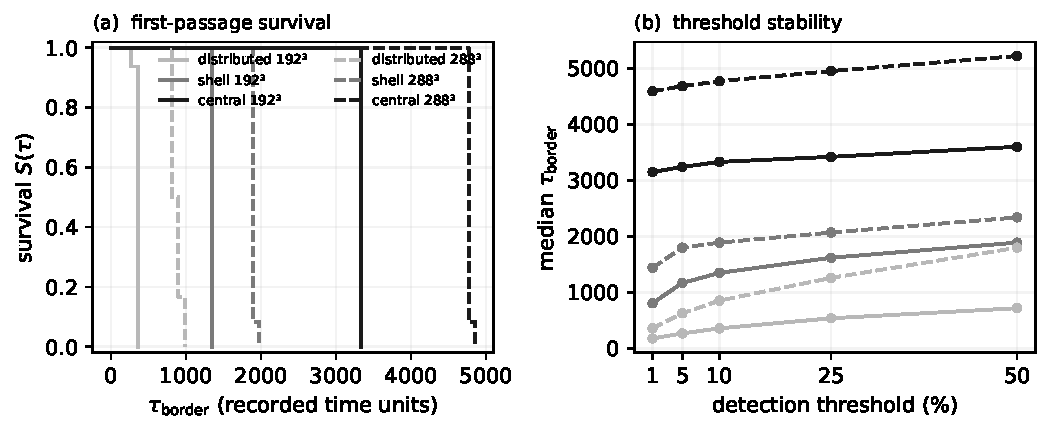
\includegraphics[width=\columnwidth]{figure1.pdf}
\caption{\label{fig:main}(a) Kaplan--Meier survival curves of $\tb$ at the \SI{10}{\percent} threshold for the three seeding topologies at both grid resolutions (solid: $192^3$; dashed: $288^3$). The three topologies separate cleanly, with the $288^3$ curves shifted to larger $\tb$. (b) Median $\tb$ as a function of detection threshold; the ordering distributed $<$ shell $<$ central holds across the full \SIrange{1}{50}{\percent} range without crossings.}
\end{figure}

\section{Discussion}
\label{sec:discussion}

\subsection{Physical interpretation}
\label{sec:physinterp}

The observed ordering admits a direct geometric interpretation. The distributed topology places seeded structure within and near the boundary shell at $t=0$, so the near-boundary gradient dissipation rises as soon as local patterns develop. The central topology requires structure to traverse the full domain radius by front propagation before it reaches the measurement shell. The shell topology, seeded close to but not within that shell, lies between. The scale ratio of $1.40$ for the fraction-preserving arm~$\mathrm{B}'$---squarely within the pre-registered bounds and far from homogenization---is consistent with self-similar scaling for the shell topology in the mid-transient. However, the onset-time decomposition of Sec.~\ref{sec:decomposition} shows that $\tb$ is not governed by a single front speed: activation and transport proxies order the topologies differently, and the transport proxy is comparable for shell and central despite very different radial distances. The ordering thus reflects seed geometry in a broader sense than radial placement---plausibly including the surface-to-volume ratio that governs pattern activation---rather than distance alone.

In the language of the entropy-production decomposition of Falasco \textit{et al.}~\cite{falasco2018}---with the caveat that our observable is a phenomenological gradient-squared analogue rather than the rigorous diffusive entropy-production rate, and that no-flux boundaries preclude actual export across the wall---$\tb$ measures the onset time of near-boundary gradient dissipation relative to its own asymptotic level. Bridging this operational proxy to the formally consistent rate, e.g.\ via the variational Gray--Scott formulation of Liang \textit{et al.}~\cite{liang2024}, is a natural next step. Our results state: \textit{the geometry of initial structure predicts when pattern-associated gradient cost first reaches a boundary-adjacent shell, with an effect size spanning up to an order of magnitude; the onset time combines a surface-limited activation phase and a subsequent transport phase} (Sec.~\ref{sec:decomposition}). This complements the finding of Serna \textit{et al.}~\cite{serna2017} that distinct morphologies can carry identical relative entropy in stationary states: even where stationary thermodynamics is morphology-blind, the \textit{transient kinetics} of near-boundary dissipation is strongly morphology-dependent.

The relevance of this geometry--kinetics coupling extends beyond the present abstract model. In morphogenesis, boundary geometry has been shown to control topological-defect transitions that determine where lumina nucleate in the mouse embryo~\cite{guruciaga2024}, and mean-field descriptions of tissue patterning now explicitly incorporate the far-from-equilibrium production and geometric compartmentalization that our dissipative framing assumes~\cite{hernandez2026}. That seed geometry predicts the onset of near-boundary gradient dissipation in an abstract Gray--Scott system is consistent with these independent observations that spatial constraints time and place self-organization in living matter. We stress that this connection is illustrative, not evidential: the present model contains no biological ingredients, and these parallels motivate the framing rather than demonstrate transferability of the result to tissues or to adaptive dynamics.

\subsection{Relation to dissipation-driven organization}

The ordering---more spatially distributed configurations reach the near-boundary dissipation threshold earlier---is qualitatively consistent with the broader program relating structure formation to dissipation enhancement, including England's dissipation-driven adaptation~\cite{england2013}. We stress the limits of this connection: our observable is a transient first-passage time, not a stationary dissipation rate, and our simulations involve no selection or adaptation dynamics. A direct test in this framework would compare long-time dissipation rates across topologies in the quasi-stationary regime---a separate study for which the present pipeline is suited but which we have not performed. The activation/transport decomposition reported here is a first step in that direction, isolating the phase most plausibly linked to dissipative structure development.

\subsection{Limitations}

Seven limitations deserve explicit statement. First, the shell--distributed contrast (990 time units) exceeds the parametric sensitivity yardstick (630) by only $1.57\times$ and is therefore weak relative to parameter uncertainty; the claim that geometry outweighs working-point sensitivity is strong only for the two contrasts involving the central topology. Second, arm~C confounds domain scale with seeded fraction (\SI{5.7}{\percent} $\to$ \SI{3.8}{\percent}); the fraction-preserving control exists only for the shell topology (arm~$\mathrm{B}'$), so ``self-similar scaling'' is established for shell alone, and the anomalous distributed ratio ($2.25$) is interpreted, but not isolated, as a fraction effect. Third, the seeding topologies differ simultaneously in radial distance, interfacial area, component number, surface-to-volume ratio, and curvature; the present design does not disentangle these, so the result supports the claim that \textit{selected initial geometries predict the onset time}, not that any single geometric variable is an independent control parameter. Fourth, the sensitivity yardstick rests on a single seed and single topology; a factorial design over seeds, topologies, and $(F,k)$ would sharpen the comparison. Fifth, all results pertain to one working point ($F=0.042$, $k=0.062$) of one model; the strong $k$-dependence observed in the probe suggests the picture should be re-examined across the Gray--Scott phase diagram before any claim of generality. Sixth, the detection threshold is normalized to each run's final value at a finite horizon $T$; for topologies that have not reached quasi-stationarity by $T$ this couples the onset time weakly to the late dynamics, and a threshold referenced to an independently defined level would be more robust. Seventh, $\tb$ is a composite observable: the decomposition of Sec.~\ref{sec:decomposition} shows it mixes a surface-limited activation phase with a subsequent transport phase that order the topologies differently, the transport proxy combines two observables on different fields, and---because the boundary is reflecting---no material is exported across it. The reported ordering is robust and reproducible, but its mechanistic attribution to ``transport'' in the strict sense is provisional and is deferred to a companion study with front tracking and absorbing boundaries.

\subsection{Outlook}

The most direct next step is to record the front position---the maximal radius at which $v$ exceeds threshold---during integration, enabling a clean separation of activation and transport and a direct test of the constant-speed model that the fill-based decomposition rejects. Beyond this, three extensions follow naturally. A self-similar arm~C (fraction-preserving seeding for all topologies) would close the confound of Sec.~\ref{sec:fullc}. A cumulative-flux variant of the observable, $\tau_{\mathrm{flux}}$---first passage of integrated boundary dissipation---can be computed from existing raw data and would test robustness to the observable definition. Finally, replacing the reflecting (no-flux) boundary with an absorbing one would probe whether the topological ordering survives when exported structure is irreversibly removed---a minimal model of asymmetric boundaries in dissipative systems. Because the pipeline records both the gradient-squared dissipation and the reaction throughput $uv^2$ per region, an operational analogue of the full diffusive/reactive entropy-production split of Falasco \textit{et al.}\ can be assembled from existing raw data, offering a route to test the thermodynamic phase-transition picture in the spherical transient regime.

\section{Conclusions}

In a three-dimensional Gray--Scott system on a spherical domain with no-flux boundaries, the spatial geometry of equal-volume initial seeding predicts the first passage of a near-boundary gradient-dissipation proxy. The ordering distributed $<$ shell $<$ central spans up to an order of magnitude in median $\tb$, replicates across two grid resolutions and independent seed batches, and is stable across threshold choices; the shell topology scales self-similarly within pre-registered bounds. The two contrasts involving the central topology exceed parametric working-point sensitivity by factors of \numrange{3}{5}, while the shell--distributed contrast is weak relative to that uncertainty. The simulations thus show a robust association between seed geometry and the onset of a boundary-adjacent gradient-dissipation proxy under the specified Gray--Scott protocol. We frame this within Prigogine's dissipative-structure program as a controlled numerical observation---not a demonstration of transport across the boundary, which the no-flux condition precludes and which a companion study with absorbing boundaries and explicit front tracking will address.

\begin{acknowledgments}
The author thanks the Kaggle platform for computational resources (dual NVIDIA T4 GPUs). This work was developed with substantial editorial, analytical, and software-engineering assistance from Anthropic's Claude (models Sonnet~4.6 and Opus~4.7), used for code review, statistical methodology discussions, literature triage, and manuscript structuring. All scientific decisions---hypothesis, frozen criteria, working-point ratification, verdict interpretation---are the author's own, as documented in the public audit trail.
\end{acknowledgments}

\appendix

\section{Numerical and statistical details}
\label{app:laplacian}

\subsection{Masked-Laplacian discretization and equivalence gate}

The spherical domain is represented as a binary mask $M(\mathbf{r})$ on the cubic grid, with $M=1$ inside the inscribed sphere and $M=0$ outside. No-flux (Neumann) boundary conditions are enforced by evaluating the Laplacian only over interior neighbors: contributions from neighbors with $M=0$ are replaced by the central value, equivalent to a reflecting boundary at the voxel level. The stencil is implemented as a single 3D convolution with a boundary-corrected kernel plus a per-site correction proportional to the number of masked neighbors, precomputed once per grid. This formulation replaces the twelve shifted-array operations of the reference implementation with one fused kernel and enables graph compilation. Numerical equivalence between the two implementations was verified as a hard gate before any production run: after 1000 steps from identical initial conditions on the target hardware, the maximum absolute field difference was $1.79\times10^{-7}$, below the pre-set tolerance of $10^{-6}$. The reference implementation and the equivalence test are retained in the repository as audit artifacts.

\subsection{Horizon rule}

The recording horizon scales with grid size (CRITERIA~v2 \S7): the state is recorded every 500 integration steps, which at $dt=0.18$ corresponds to 90 time units, giving a horizon of $T=8100$ recorded units at $192^3$ (45\,000 steps, 91 records) and $T=12\,060$ at $288^3$ (67\,000 steps, 135 records). The observable $\tb$ is quantized to this recording grid: it is returned as the first recorded time at which the threshold is met, without interpolation between records. All raw per-run $\tb$ values are therefore multiples of 90, and each carries a quantization uncertainty of $\pm45$ time units; reported medians at even $n$ (e.g.\ 855 for distributed at $288^3$) can fall between grid points as the mean of two adjacent order statistics ($810$ and $900$). The scaling keeps the horizon proportional to the domain radius, so front-propagating structure has commensurate time to reach the boundary at both resolutions. A run whose boundary dissipation never reaches threshold within $T$ is right-censored rather than discarded.

\subsection{Seeding construction}

All topologies seed on a background of the trivial state $u=1$, $v=0$; seeded voxels are set to $u=0.5$, $v=0.25$, with uniform noise of amplitude $0.02$ added to $v$ inside the seeded region only. The shell topology sets the seeding budget: a spherical layer of prescribed thickness (default $3.0$ voxels; $4.5$ in the self-similar $\mathrm{B}'$ variant) is built at radius $0.75R$, and its voxel count $N_{\mathrm{target}}$ defines the target for the other two topologies. The \textit{central} mask is a centered ball whose radius is matched to $N_{\mathrm{target}}$ by 60-iteration bisection; the \textit{distributed} mask accumulates the union (not the sum) of small random balls---radius $\max(2.0, 0.03n)$ voxels, placed by rejection sampling---until the union reaches $N_{\mathrm{target}}$. Matching the union rather than summing blob volumes makes the volume match hold in the presence of overlap. The seeded fraction is therefore geometry-forced and identical across topologies (${\approx}\SI{5.7}{\percent}$ at $192^3$ with thickness $3.0$; ${\approx}\SI{3.8}{\percent}$ at $288^3$), and is recorded in run metadata rather than assumed, since it is resolution-dependent. The topologies differ in how much the seed geometry varies between runs: the \textit{central} and \textit{shell} masks are deterministic functions of the grid, so only the additive $v$-noise differs between seeds, whereas the \textit{distributed} mask draws fresh blob centers from the per-seed random stream and thus realizes a genuinely different geometry each run. Consequently the number of independent geometric realizations equals $n$ only for the distributed topology; for central and shell the between-run variation is confined to the noise field, which (Sec.~\ref{sec:results}) leaves $\tb$ essentially unchanged.

\subsection{Seeding admissibility gates}
\label{app:gates}

Because $\tb$ measures the arrival of structure at the boundary shell $r\in[0.85R,R]$, any seed placed inside that shell would pre-load the observable. Two geometric gates, frozen with the rest of the protocol, prevent this. Gate B4 requires zero seeded voxels within the measurement shell; distributed blobs are constrained entirely below $0.85R$ by construction. Gate B5 caps the outermost seeded radius of the \textit{central} ball at $0.40R$---$0.8\times$ the inner-core radius ($0.5R$)---so the central seed cannot engulf the interior measurement region and change the meaning of the observable relative to the other topologies; this simultaneously bounds the admissible seeded fraction at ${\le}\SI{6.4}{\percent}$. Both gates are evaluated and logged per run. These controls were introduced after a pilot in which seeds overlapping the measurement shell produced a nonzero boundary dissipation at $t=0$ for the distributed topology alone, disqualifying first-passage comparison (see repository FINDINGS).

\subsection{Survival analysis}

For each topology pair we compare Kaplan--Meier survival curves of $\tb$ with the Mantel--Cox log-rank statistic, treating runs that never reach threshold as events beyond horizon. The three pairwise $p$-values per arm are Holm-corrected within the full family of comparisons across both arms (six tests). Median confidence intervals are obtained from the Kaplan--Meier estimator; non-overlap is reported as a secondary check. Mann--Whitney $U$ on raw $\tau$ values is reported only as a cross-check where censoring is absent, as it assigns no rank to a non-event.

\subsection{Dissipation and reaction fields}

Per-voxel fields are computed as $D(\mathbf{r}) = D_u|\nabla u|^2 + D_v|\nabla v|^2$ (gradient-squared dissipation analogue) and $R(\mathbf{r}) = uv^2$ (reaction throughput), with gradients evaluated by the same masked stencil as the Laplacian. Region averages over the inner core ($r\le0.5R$) and boundary shell ($r\in[0.85R,R]$) yield the inner and boundary dissipation and reaction densities. Following the model's phenomenological status, these are dissipation \textit{analogues}: Gray--Scott is not a thermodynamically consistent reaction network, and $|\nabla\cdot|^2$ is not the rigorous entropy-production rate. They are nonetheless well-defined, topology-comparable cost densities, and their boundary values define the primary observable $\tb$.

\begin{table*}[htbp]
\caption{\label{tab:logrank}Pairwise log-rank (Mantel--Cox) contrasts of $\tb$ between seeding topologies, at both grid resolutions. Medians in recorded time units; $p_{\mathrm{Holm}}$ is Holm-corrected across the six-test family. All confidence intervals non-overlapping; no censored runs.}
\begin{ruledtabular}
\begin{tabular}{llcccc}
Arm & Contrast & Median (a vs b) & $\chi^2$ & $p$ & $p_{\mathrm{Holm}}$ \\
\colrule
A ($192^3$) & central vs shell & 3330 / 1350 & 31.00 & $2.6\times10^{-8}$ & $1.5\times10^{-7}$ \\
A ($192^3$) & central vs distributed & 3330 / 360 & 30.22 & $3.9\times10^{-8}$ & $1.9\times10^{-7}$ \\
A ($192^3$) & shell vs distributed & 1350 / 360 & 30.22 & $3.9\times10^{-8}$ & $1.9\times10^{-7}$ \\
C ($288^3$) & central vs shell & 4770 / 1890 & 25.38 & $4.7\times10^{-7}$ & $1.3\times10^{-6}$ \\
C ($288^3$) & central vs distributed & 4770 / 855 & 25.55 & $4.3\times10^{-7}$ & $1.3\times10^{-6}$ \\
C ($288^3$) & shell vs distributed & 1890 / 855 & 25.55 & $4.3\times10^{-7}$ & $1.3\times10^{-6}$ \\
\end{tabular}
\end{ruledtabular}
\end{table*}

\begin{table}[htbp]
\caption{\label{tab:threshold}Median $\tb$ as a function of the detection threshold (fraction of final value), at both resolutions. The ordering distributed $<$ shell $<$ central holds at every threshold on both grids.}
\begin{ruledtabular}
\begin{tabular}{lcccccc}
& \multicolumn{3}{c}{$192^3$ (A)} & \multicolumn{3}{c}{$288^3$ (C)} \\
\cline{2-4}\cline{5-7}
Thr. & central & shell & distr. & central & shell & distr. \\
\colrule
\SI{1}{\percent}  & 3150 & 810  & 180 & 4590 & 1440 & 360 \\
\SI{5}{\percent}  & 3240 & 1170 & 270 & 4680 & 1800 & 630 \\
\SI{10}{\percent} & 3330 & 1350 & 360 & 4770 & 1890 & 855 \\
\SI{25}{\percent} & 3420 & 1620 & 540 & 4950 & 2070 & 1260 \\
\SI{50}{\percent} & 3600 & 1890 & 720 & 5220 & 2340 & 1800 \\
\end{tabular}
\end{ruledtabular}
\end{table}

\begin{table}[htbp]
\caption{\label{tab:yardstick}Inter-topology differences in median $\tb$ at $192^3$, compared against the parametric sensitivity yardstick (spread of $\tb$ under $(F,k)\pm\SI{0.5}{\percent}$, in-regime).}
\begin{ruledtabular}
\begin{tabular}{lcc}
Quantity & Value (steps) & Ratio to yardstick \\
\colrule
Yardstick: $(F,k)\pm\SI{0.5}{\percent}$ spread & 630 & $1.0\times$ (ref.) \\
central $-$ distributed & 2970 & $4.7\times$ \\
central $-$ shell & 1980 & $3.1\times$ \\
shell $-$ distributed & 990 & $1.57\times$ \\
\end{tabular}
\end{ruledtabular}
\end{table}

\begin{table}[htbp]
\caption{\label{tab:decomp}Decomposition of the onset time at $192^3$. Activation proxy $t_{\mathrm{act}}$ is the median time to reach normalized fill $\tilde\phi=\SI{10}{\percent}$; transport proxy $t_{\mathrm{tr}}=\tb-t_{\mathrm{act}}$. Seed mass-center radius is given for reference. All times in recorded units.}
\begin{ruledtabular}
\begin{tabular}{lcccc}
Topology & mass-center & $t_{\mathrm{act}}$ & $\tb$ & $t_{\mathrm{tr}}$ \\
\colrule
distributed & ${\approx}0$ & 180 & 360 & 180 \\
shell & $0.75R$ & 90 & 1350 & 1260 \\
central & $0$ & 2250 & 3330 & 1080 \\
\end{tabular}
\end{ruledtabular}
\end{table}

\begin{thebibliography}{99}

\bibitem{prigogine1977} G.~Nicolis and I.~Prigogine, \textit{Self-Organization in Nonequilibrium Systems} (Wiley, New York, 1977).
\bibitem{nicolis1971} G.~Nicolis and I.~Prigogine, Proc. Natl. Acad. Sci. USA \textbf{68}, 2102 (1971).
\bibitem{cross1993} M.~C.~Cross and P.~C.~Hohenberg, Rev. Mod. Phys. \textbf{65}, 851 (1993).
\bibitem{falasco2018} G.~Falasco, R.~Rao, and M.~Esposito, Phys. Rev. Lett. \textbf{121}, 108301 (2018).
\bibitem{liang2024} J.~Liang, N.~Jiang, C.~Liu, Y.~Wang, and T.~Zhang, arXiv:2409.04663 (2024).
\bibitem{serna2017} H.~Serna, A.~P.~Mu\~nuzuri, and D.~Barrag\'an, Phys. Chem. Chem. Phys. \textbf{19}, 14401 (2017).
\bibitem{bak1987} P.~Bak, C.~Tang, and K.~Wiesenfeld, Phys. Rev. Lett. \textbf{59}, 381 (1987).
\bibitem{grebenkov2020} D.~S.~Grebenkov, J. Phys. A: Math. Theor. \textbf{53}, 445601 (2020).
\bibitem{grebenkov2022} D.~S.~Grebenkov, J. Phys. A: Math. Theor. \textbf{55}, 235201 (2022).
\bibitem{pearson1993} J.~E.~Pearson, Science \textbf{261}, 189 (1993).
\bibitem{gray1984} P.~Gray and S.~K.~Scott, Chem. Eng. Sci. \textbf{39}, 1087 (1984).
\bibitem{england2013} J.~L.~England, J. Chem. Phys. \textbf{139}, 121923 (2013).
\bibitem{degroot1984} S.~R.~de~Groot and P.~Mazur, \textit{Non-Equilibrium Thermodynamics} (Dover, New York, 1984).
\bibitem{kaplan1958} E.~L.~Kaplan and P.~Meier, J. Am. Stat. Assoc. \textbf{53}, 457 (1958).
\bibitem{mantel1966} N.~Mantel, Cancer Chemother. Rep. \textbf{50}, 163 (1966).
\bibitem{holm1979} S.~Holm, Scand. J. Stat. \textbf{6}, 65 (1979).
\bibitem{villarsepulveda2024} E.~Villar-Sep\'ulveda, A.~R.~Champneys, D.~Cusseddu, and A.~Madzvamuse, arXiv:2409.06826 (2024).
\bibitem{bentahar2023} S.~Ben~Tahar, J.~J.~Mu\~noz, S.~J.~Shefelbine, and E.~Comellas, bioRxiv 10.1101/2023.03.29.534782 (2023).
\bibitem{kobayashi2026} S.~Kobayashi, K.~Sakakibara, and T.~Uechi, arXiv:2601.04746 (2026).
\bibitem{guruciaga2024} P.~C.~Guruciaga, T.~Ichikawa, S.~Plunder, T.~Hiiragi, and A.~Erzberger, arXiv:2403.08710 (2024).
\bibitem{hernandez2026} D.~Hern\'andez, A.~Vald\'es~L\'opez, and E.~C.~Herrera-Hern\'andez, arXiv:2606.10355 (2026).

\end{thebibliography}

\end{document}
